%!TEX root = ../Master.tex
\section{Discussion}\label{sec:discussion}

% rate adaptation
% similar drops , no use in changing, policy -> don't change rate, for this specific scenario - others where the drone is further away might benefit
It is seen in Figure \ref{fig:trace} that the four TxR experience a similar PER over time. Since the PERs are correlated the 36 Mb/s TxR offers the highest throughput and the best adaptation policy is to select the highest TxR. We remind the reader that this policy is suitable for the specific scenario described in Section \ref{sec:methodmaterials}. In scenarios with other environments and longer distance between sender and receiver this might not be the optimal policy. This limits our adjustment policy to RLNC and video rate.

% network coding
%RLNC, is used to deal with packet erasure, and still get same throughput, by sending redundant information, green line in figure, red line included as 1 second average, because its rarely completely lost connection
RLNC is used to add redundancy to the transmitted video. This allows recovery of the transmitted video at the receiver if the amount of redundancy is equal to or greater than the PER. Since we assume instant feedback, the optimal RLNC policy is to add redundancy equivalent to the PER. The green curve in Figure \ref{fig:delay}(a) illustrates the available throughput to the video rate of a 8.8 minutes trace. The throughput is based on the estimation presented in Figure \ref{fig:trace}. Because the trace can fluctuate aggressively, the trace is overlaid by a red line, which is the average throughput over the last second. From this red line, we see that the available throughput rarely drops to 0 Mb/s. From Figure \ref{fig:delay}(a) and Figure \ref{fig:vtrace} we calculate the time it takes to send a frame
from when it was captured till it has reached the receive buffer.
This is calculated for each individual frame and can be seen as the blue bars in Figure \ref{fig:delay}(b,c,d), we denote this as the per frame delay. This delay introduces the playback delay which is the time between a frame is taken until it is displayed at the receivers. A playback freeze occurs when the next frame is delayed beyond the current playback delay. Depending on the playback method these metrics have different impacts.\\
% playback freezes when a frame is delayed. Frame delay = playback freeze, playback freezes can be seen on Fig delay - horisontal applyes to delaybounded, horizontal applies to continuous
\textbf{Continuous} playback is playing every frame of the video in chronological order. Whenever a frame is delayed more than the previous frame the playback delay is increased and a playback freeze occurs. The red dotted lines in Figure \ref{fig:delay}(b,c,d,e) illustrate the playback delay. These freezes can be seen as small vertical boxes on the far right in Figure \ref{fig:delay}(b,c,d,e). The strength is that every frame of the video is present, the weakness is that there is no upper bound on either the playback delay, or the buffer size. This method accumulates the delay whenever a freeze occurs, which means that the receivers will eventually be heavily unsynchronized with the sender.  \\
%
\textbf{Delay bounded} playback sets a strict delay requirement and this is the exact amount of time before the receiver will play the video, this is illustrated as the black dotted line in Figure \ref{fig:delay}(b,c,d,f). Frames delayed beyond this threshold are discarded thereby guaranteeing strict delay and buffer sizes on the sender and receivers. Playback freezes occur every time a frame/series of frames are delayed beyond the threshold. The strength of this method is that the video has a constant playback delay, but the down side is freezes occur in the video whenever frames are not delivered fast enough. The delay bounded freezes are marked as small horizontal boxes under the x-axis of Figure \ref{fig:delay}(b,c,d,f).

\begin{figure}[ht]
  	\centering
  	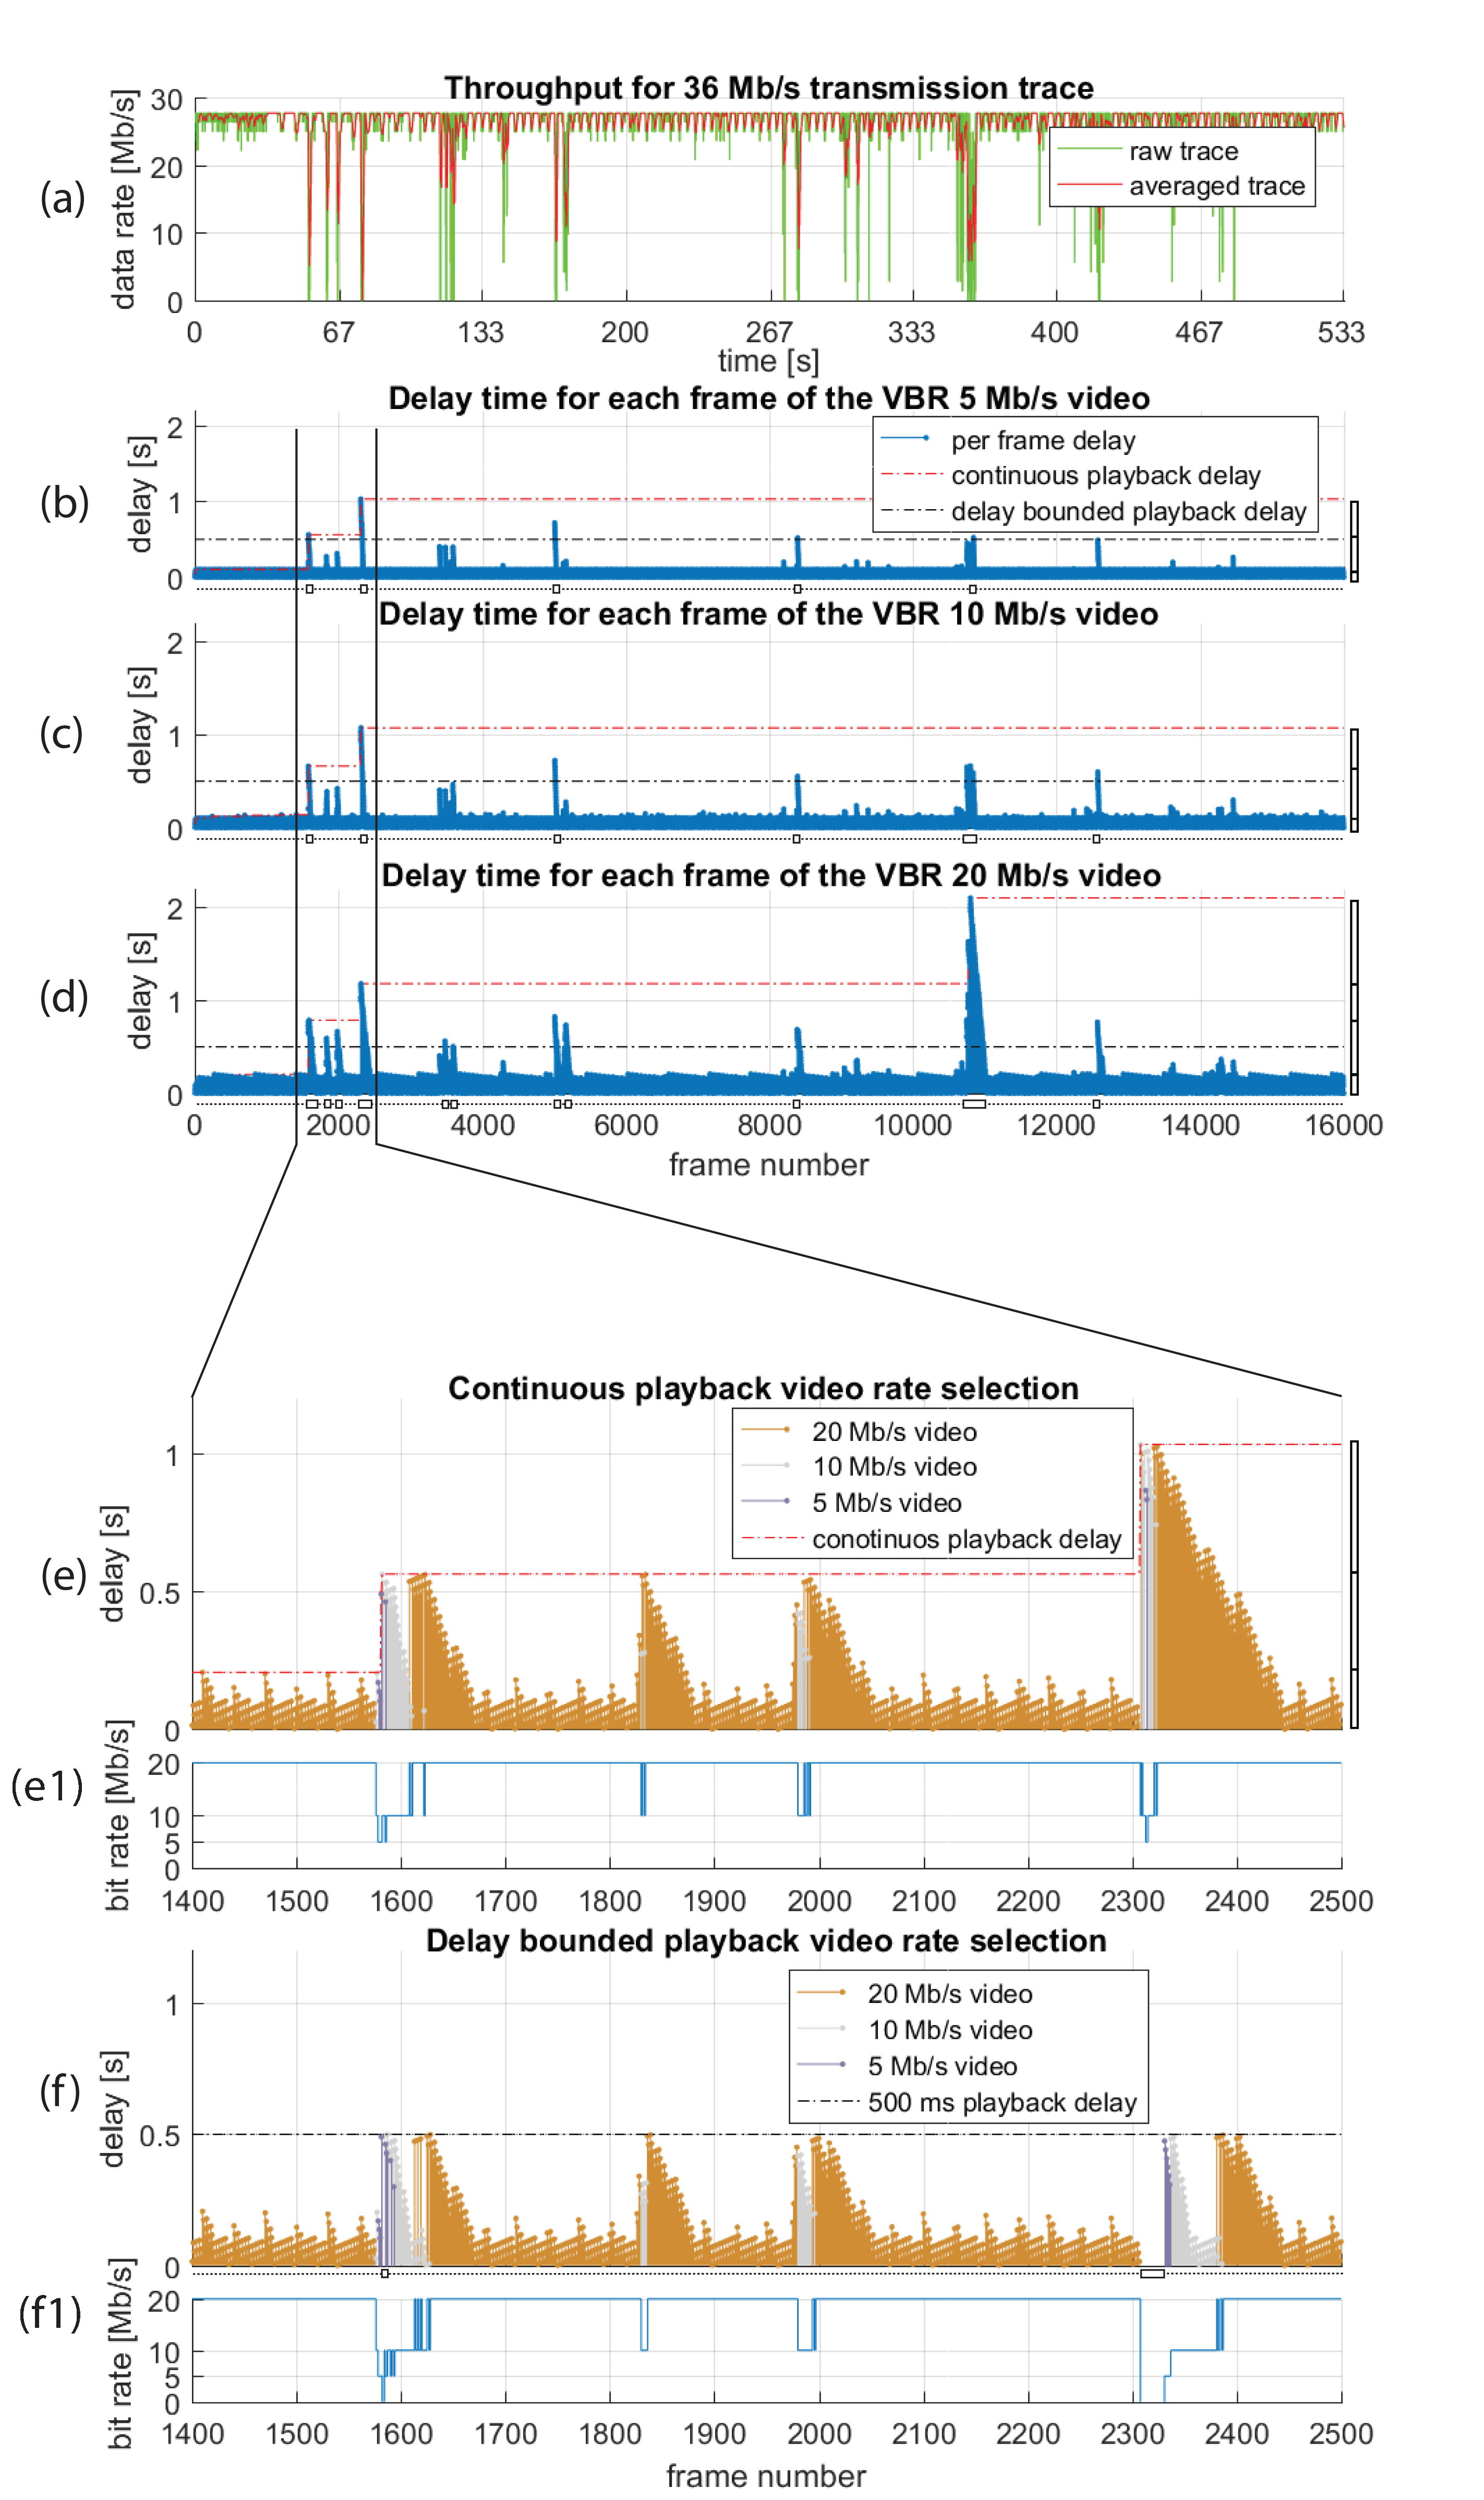
\includegraphics[width=\linewidth]{images/LargeImage.pdf}
  	\caption{Correlation between frame delay and the network condition}
  	\label{fig:delay}
\end{figure}

Common for both playback methods is that they will experience playback freezes if the delay of certain frames is large. In Table \ref{tbl:videos} are the number of freeze periods and combined freeze time for each video rate. Note that the delay bounded playback is set to 500 ms in our analysis. If the delay bound is set to 1 s less freezes occurs.
\begin{table}[]
\centering
\begin{tabular}{c|c|c|c|c|}
\cline{2-5}
\multicolumn{1}{r|}{}                                                                                    & Video Rates                                                                               & 5 Mb/s                       & 10 Mb/s                      & 20 Mb/s                      \\ \hline
\multicolumn{1}{|c|}{\multirow{3}{*}{\begin{tabular}[c]{@{}c@{}}Continuous \\ playback\end{tabular}}}                                                        & Playback freezes                                                                          & 3                            & 3                            & 4                            \\ \cline{2-5}
\multicolumn{1}{|c|}{}                                                                                   & Total freeze time                                                                         & 1.032 s                      & 1.074 s                      & 2.102 s                      \\ \cline{2-5}
\multicolumn{1}{|c|}{}                                                                                   & \multicolumn{1}{l|}{\begin{tabular}[c]{@{}l@{}}Accumulated\\ playback delay\end{tabular}} & \multicolumn{1}{l|}{1.032 s} & \multicolumn{1}{l|}{1.074 s} & \multicolumn{1}{l|}{2.102 s} \\ \Cline{1-5}{1.5pt}
\multicolumn{1}{|c|}{\multirow{3}{*}{\begin{tabular}[c]{@{}c@{}}Delay bounded \\ playback\end{tabular}}} & Playback freezes                                                                          & 5                            & 6                            & 11                           \\ \cline{2-5}
\multicolumn{1}{|c|}{}                                                                                   & Total freeze time                                                                         & 1.133 s                      & 2.533 s                      & 15.833 s                     \\ \cline{2-5}
\multicolumn{1}{|c|}{}                                                                                   & \multicolumn{1}{l|}{\begin{tabular}[c]{@{}l@{}}Accumulated\\ playback delay\end{tabular}} & \multicolumn{1}{l|}{0.5 s}   & \multicolumn{1}{l|}{0.5 s}   & \multicolumn{1}{l|}{0.5 s}   \\ \hline
\end{tabular}
\caption{Comparison of certain metrics in video playback}
\label{tbl:videos}
\end{table}

For the 20 Mb/s video we see that if continues playback is used, we experience 4 freezes and that the total freeze time is approximately 2 seconds. If bounded playback is used instead we will experience 11 freeze periods which accumulate to approximately 16 seconds. Similar numbers for the other video rates can be seen in Table \ref{tbl:videos}.

Even though the 20 Mb/s video experiences greater delay than the lower quality videos these delays only occur for a fraction of the frames recorded. This means that is is possible to use the 20 Mb/s video for the majority of the stream. By adjusting the video rate when frame delay is high it is possible to reduce playback delay and the number of freeze periods in the  live video stream.

%way of adjusting video rate to minimize delay.
We propose two ways of adjusting the video rate depending on the playback method used. For continuous playback an initial playback delay is introduced. Whenever a frame is delayed beyond the initial delay we switch to the video rate which causes the lowest additional delay. If the delay decreases, we switch to the highest video rate that does not introduce further delay. An illustration of this policy is seen in Figure \ref{fig:delay}(e) where the different colours denote which video rate was used on the frame and \ref{fig:delay} (e1) shows the video rate. We see that if this policy is applied on the traces it switches incorrectly in some cases, this is because the captured videos are not identical.

For the delay bounded method the policy is as follows: as long as frames from the 20 Mb/s video are delayed less than 500 ms they are played. If the delay is exceeded a lower video rate that still fulfil the requirements is used. If none of the video rates are able to fulfil the 500 ms delay requirement we experience playback freeze. Figure \ref{fig:delay}(f) illustrates the switching done to fulfil the 500 ms delay requirement and Figure \ref{fig:delay}(f1) shows the video rate. When the video rate drops to 0 Mb/s a playback freeze period occurs.

% general discussion
These two policies give better performance for both playback methods in terms of number of freezes and freeze time. The methods are inherently different, so choosing a method depends on the desired playback delay and the application of the video.
%Continuous playback gives fewer freezes and lower freeze time, but the overall playback delay accumulates. Delay bounded playback guarantees a constant playback delay, but experience more freezes and longer freeze time.



%Figure \ref{fig:comb_trace} contains a segment of the goodput trace for 36 Mb/s along with the trace of the necessary Network coding %overhead in order to protect the video feed against packet loss, the network coding trace is under the assumption of instantaneous %feedback, no coding delay and no network coding overhead. The amount of network coding added is determined from the goodput of %approximately 27 Mb/s and the loss trace where redundancy is added based on the losses and the available bandwidth for video data is %obtained as area under the blue curve.
%By examining the segment it is seen that for the most part it is possible to deliver the video to the users without problem. However at a %certain point the packet loss becomes too great for the link to sustain the 20 Mb/s video stream and a lower bit rate for the video must %be used in these cases.
%In order to sustain the spikes of the video it is necessary to spread them across the remaining period before the next I-frame. Depending %on the size of the I-frame in the trace and the delay of the stream will change, since a fully receive I-frame is necessary in order to %decode the video. The delay requirement is therefore also something that should be taken into account when adjusting the video and %Network Coding. If the goodput with network coding approaches the goodput rate the delay increases as there is less extra bandwidth for %quickly transmitting the I-frame, and one should preferably change the video rate to stay at or below the acceptable video delay.
%
%
%Figure \ref{fig:delay} shows the per frame delay of the three different video data rates. The 20 Mb/s video has a maximum delay of 2.1s, %the 10Mb/s has a maximum delay of 1.08s and the 5Mb/s has a maximum of 1.03s. It is remarkable that some of the delay spikes are very %similar across the different data rates, while others are significantly different. By overlaying a moving average MA(25) of the network %data rate we observe that when the data rate curve has a very steep slope, the delay response of the different videos are similar, while %when the slope is just moderately steep, the delay is significantly worse for the high bit rate videos.
%
%If one were to set the playback delay at the receiver to 500ms (discard any frames that are older than 500ms) the video would experience %freeze periods followed by a jump in the video, when the video picks up again. The number of freezes for the three video bit rates are: %5Mb/s video causes 5 freezes, 10Mb/s video causes 6 freezes and 20Mb/s causes 10 freezes. I.e. if a 500ms playback delay was desired we %can use the 20 Mb/s video bit rate for the majority of the time, but limit the number of freezes to 5 (instead of 10), by decreasing the %video bit rate 5 times.
